\documentclass{beamer}
\usepackage[utf8]{inputenc}
\usepackage[T1]{fontenc}

\usepackage{amsmath}
\usepackage{mathtools}
\usepackage{amsthm}
\usepackage{amssymb}
\usepackage{tcolorbox}
\tcbuselibrary{theorems}
\usepackage{tikz-cd}
\usepackage{xparse}
\usepackage{adjustbox}



%\newcommand{\cat}[1]{\mathcal{#1}}

\usepackage{pst-text}




\title{A Frobenius and Hopf Algebraic Formulation of Quantum Field Theory}

\author{Matt Alexander}
\usetheme{queer}


%\newcommand{\newthought}[1]{\medskip\noindent\fbox{{#1}}}




%=================================
% Colourblind-friendly colours
%=================================


% 6 Colour Attempt Feb 27, 2024


\definecolor{lemmacolour}{RGB}{0, 0, 153} 


\definecolor{propcolour}{RGB}{138, 10,0}

\definecolor{definitioncolour}{RGB}{100, 100, 100}

\definecolor{examplecolour}{RGB}{62,217,141}

\definecolor{conjecturecolour}{RGB}{235, 160, 215}

\definecolor{theoremcolour}{RGB}{255, 240, 0}



%============================
% 5 Colour Attempt
%============================



%\definecolor{corolcolour}{RGB}{0, 114, 178}


%Compare this one and examplecolor on tritanopia
%\definecolor{lemmacolour}{RGB}{0, 114, 178} 
%
%
%\definecolor{propcolour}{rgb}{0.6, 0.0,0.0}
%
%
%\definecolor{theoremcolour}{rgb}{1.0, 0.84, 0.0}
%
%
%
%
%\definecolor{examplecolour}{RGB}{59,191,143}
%
%\definecolor{definitioncolour}{rgb}{0.75, 0.75, 0.75}



%============================
% Theorem Environments
%============================


\usepackage{}



\newenvironment{proof-lemma}
    {\begin{mdframed}[linewidth=3, linecolor=lemmacolour,topline=false,rightline=false,bottomline=false]
\begin{proof}
}{
\end{proof}
\end{mdframed}}


\newenvironment{proof-prop}
    {\begin{mdframed}[linewidth=3, linecolor=propcolour,topline=false,rightline=false,bottomline=false]
\begin{proof}
}{
\end{proof}
\end{mdframed}}


\newenvironment{proof-theorem}
    {\begin{mdframed}[linewidth=3, linecolor=theoremcolour,topline=false,rightline=false,bottomline=false]
\begin{proof}
}{
\end{proof}
\end{mdframed}}

\newenvironment{proof-corol}
    {\begin{mdframed}[linewidth=3, linecolor=lemmacolour,topline=false,rightline=false,bottomline=false]
\begin{proof}
}{
\end{proof}
\end{mdframed}}

\newenvironment{defframe}
    {\begin{mdframed}[linewidth=3, linecolor=definitioncolour,topline=false,rightline=false,bottomline=false]
}{
\end{mdframed}}

\newenvironment{exampleframe}
    {\begin{mdframed}[linewidth=3, linecolor=examplecolour,topline=false,rightline=false,bottomline=false]
}{
\end{mdframed}}

\newenvironment{conjecframe}
    {\begin{mdframed}[linewidth=3, linecolor=conjecturecolour,topline=false,rightline=false,bottomline=false]
}{
\end{mdframed}}



%============================

%\newtcbtheorem[number within=section]{theorem}{\color{black}Theorem}%
%{colback=theoremcolour!5,colframe=theoremcolour,fonttitle=\bfseries}{th}





%==========================================



%==============================================
% Theorems v.2
%==============================================


\newtcbtheorem[number within=section]{deff}{Definition}%
{colback=definitioncolour!5, colframe=definitioncolour,fonttitle=\bfseries}{th}


\newtcbtheorem[number within=section]{lemm}{Lemma}%
{colback=lemmacolour!5,colframe=lemmacolour!95!black,fonttitle=\bfseries}{th}



% Had to change this just for this presentation, so we didn't get prop 0.1, since there are no 'sections' in a beamer presentation.

\newtcbtheorem{prop}{Proposition}%
{colback=propcolour!5,colframe=propcolour,fonttitle=\bfseries}{th}



\newtcbtheorem[number within=section]{corol}{Corollary}%
{colback=corolcolour!5,colframe=corolcolour!95!black,fonttitle=\bfseries}{th}

\newtcbtheorem[number within=section]{exam}{Example}%
{colback=examplecolour!5,colframe=examplecolour,{fonttitle=\bfseries \color{black}}}{th}



\newtcbtheorem[number within=section]{conj}{Conjecture}%
{colback=conjecturecolour!5,colframe=conjecturecolour,{fonttitle=\bfseries \color{black}}}{th}


\newtcbtheorem[number within=section]{thm}{\color{black}Theorem}%
{colback=theoremcolour!5,colframe=theoremcolour,{fonttitle=\bfseries \color{black}},
label type=theorem}{thm}



%==============================================
% Theorems v.1
%==============================================


%\newtcbtheorem[number within=section]{definition}{Definition}%
%{colback=definitioncolour!5,colframe=definitioncolour!50!black,fonttitle=\bfseries}{th}
%
%
%\newtcbtheorem[number within=section]{lemma}{Lemma}%
%{colback=lemmacolour!5,colframe=lemmacolour!95!black,fonttitle=\bfseries}{th}
%
%
%\newtcbtheorem[number within=section]{prop}{Proposition}%
%{colback=propcolour!5,colframe=propcolour,fonttitle=\bfseries}{th}
%
%
%
%\newtcbtheorem[number within=section]{corollary}{Corollary}%
%{colback=corolcolour!5,colframe=corolcolour!95!black,fonttitle=\bfseries}{th}
%
%\newtcbtheorem[number within=section]{example}{Example}%
%{colback=examplecolour!5,colframe=examplecolour!90!black,fonttitle=\bfseries}{th}
%
%
%
%\newtcbtheorem[number within=section]{conjecture}{Conjecture}%
%{colback=conjecturecolour!5,colframe=conjecturecolour!90!black,fonttitle=\bfseries}{th}
%
%
%\newtcbtheorem[number within=section]{theorem}{\color{black}Theorem}%
%{colback=theoremcolour!5,colframe=theoremcolour,{fonttitle=\bfseries \color{black}},
%label type=theorem}{thm}








%\usepackage[demo]{graphicx}
\usepackage{wallpaper}
\usepackage{wrapfig,booktabs}

\usepackage{fancyhdr}
\usepackage{lettrine}

\usepackage{mdframed}

\usepackage{cancel}

%\usepackage{geometry}
%\geometry{
%tmargin=5cm, 
%bmargin=5cm, 
%lmargin=5cm, 
%rmargin=3cm,
%headheight=1.5cm,
%headsep=0.8cm,
%footskip=0.5cm}


\usepackage{tabularx}

\usepackage{braket}




%=====================
% MATH
%=====================

\usepackage{amsmath}
\usepackage{mathtools}
\usepackage{amsthm}
\usepackage{amssymb}
\usepackage{tcolorbox}
\tcbuselibrary{theorems}
\usepackage{tikz-cd}
\usepackage{xparse}

% To get a get a nice curvy arrow to talk about paths
\DeclareSymbolFont{lasy}{U}{lasy}{m}{n}
\SetSymbolFont{lasy}{bold}{U}{lasy}{b}{n}
\DeclareMathSymbol\leadsto{\mathrel}{lasy}{"3B}



% To have arrow heads in the middle
\usetikzlibrary{decorations.markings, arrows.meta}
\tikzset{
    marrow/.style={decoration={markings,mark=at position 0.5 with {\arrow{#1}}}, postaction=decorate}
}


%\usepackage[colorlinks=true]{hyperref}

\usepackage[nameinlink]{cleveref} % Better references to lemmas etc. The nameinlink makes all of 'Theorem 1' clickable


%\usepackage{titling} %Lets you have more than one title in a document
% But this won't work with ams articles, so I'll need to add it in separately for my own work and comment it out for research articles


\usepackage{adjustbox}



\usepackage[nointegrals]{wasysym}

\usepackage{fontawesome} % really cool fonts like morph and obj
\usepackage{tikz}



%========================
% COMMANDS
%========================


\newcommand{\Def}[1]{\textbf{\boldmath{#1}}}



%Field Theory
\newcommand{\exten}[2]{{#2}_{#1}}



\newcommand{\colim}{\operatorname{colim}}

\newcommand{\tabitem}{~~\llap{\textbullet}~~}

\newcommand{\newthought}[1]{\medskip\noindent\fbox{{#1}}}


\newcommand{\abs}[1]{| #1 |}

\newcommand{\cat}[1]{\mathcal{#1}}


\newcommand{\coker}{\operatorname{coker}}

\newcommand{\im}{\operatorname{Im}}

\newcommand{\const}{\text{\faAsterisk}}


\newcommand{\obj}{\text{\faCube}}

\newcommand{\morph}{\text{\faLocationArrow}}

\newcommand{\mor}[2]{\text{Mor}(#1, #2)}

\newcommand{\nbh}[1]{\mathcal{N}_{#1}} % The set of neighbourhoods around $x$.


\newcommand{\twist}{\text{\faRefresh}}


%================================
% HOMOTOPY / MODEL CATEGORIES
%=================================

\newcommand{\cyl}{\text{\faDatabase}}

\newcommand{\paths}{\text{\faPencilSquareO }}


%
%\newcommand{\bnbh}[1]{\mathcal{B}_{#1}}
%
%\newcommand{\base}[1]{\langle \cdot #1 \cdot \rangle}

\newcommand{\norm}[1]{\left\lVert #1 \right\rVert}

\newcommand{\gen}[1]{\left\langle #1 \right\rangle}

\newcommand{\triforce}{\resizebox{1em}{!}{
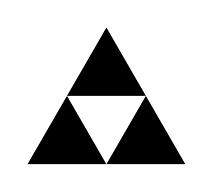
\begin{tikzpicture}
\fill[black] (0,0)  -- +(2,0) -- +(60:2) -- cycle;
\fill[white]  (60:1) -- +(1,0)  -- (1,0) -- cycle;
\end{tikzpicture}
}}





\begin{document}







%============================
% FRAME 0
%============================


\begin{frame}

\titlepage


\end{frame}
















\begin{frame}

\frametitle{Frobenius Algebras}

\framesubtitle{Definition}

%\begin{definition}
%{Graded Frobenius Algebra}{•}
A \Def{graded Frobenius $*$-algebra} $(F, \gen{\cdot, \cdot})$, is a graded not-necessarily associative nor unital algebra $F$ over a $*$-ring $k$, with non-degenerate bilinear form $\gen{\cdot, \cdot}: F \otimes F \to k$, such that
\begin{equation}
\gen{xy,z} = \gen{x,y^* z}
\end{equation}
for all $x,y,z \in F$, and for all non-zero $x \in F$, there exist some $a,b \in F$ such that $a x$ and $x b \ne 0$.
%\end{definition}

\end{frame}



%============================
% FRAME
%============================


\begin{frame}
\frametitle{Frobenius Algebras}

\framesubtitle{Examples}



\begin{tabularx}{\textwidth}{lll>{\raggedright\arraybackslash}X}
\toprule
Space & $\mu$ & $\gen{\cdot, \cdot}$ 
\\
\midrule
\\
$C_c^{\infty}(X)$ & Pointwise & $\gen{f,g} = \int f^* g$ \\
Schwartz functions $\cat{S}$ & Pointwise & $\gen{f,g} = \int f^* g$
\\
\\
$\mathbb{R}^n$ w/ basis $\{ e_i \}$ & $e_i e_j = \delta_{ij} e_i$ & $\gen{e_i,e_j} = \delta_{ij}$ \\
Hilbert space w/ basis $\{ e_i \}$ & $e_i e_j = \delta_{ij} e_i$ & $\gen{e_i,e_j} = \gen{e_i, e_j}_H$  \\
\\
$kG$ (finite group) & Group mult. & $\gen{g,h} = \delta_{gh, 1}$ 
\\
\bottomrule
\end{tabularx}

\medskip


\begin{equation*}
\cat{S} = \{ f \in C^{\infty}(\mathbb{R}^n, \mathbb{C}) \mid \sup_{x} \abs{x^\alpha D^\beta f(x)} < \infty, \forall \alpha, \beta \}
\end{equation*}



\end{frame}


%============================
% FRAME
%============================


\begin{frame}

\frametitle{Weak Topology}

\framesubtitle{Frobenius Algebra}

Let $F$ be Frobenius. We consider the coarsest topology such that the maps
\begin{equation*}
\begin{split}
F \xrightarrow{\abs{\gen{x, -} }} k \\
F \xrightarrow{\abs{ \gen{-, y}} } k
\end{split}
\end{equation*}
are continuous for all $x,y \in F$, which we call the \textbf{weak topology} on $F$

\medskip

\newthought{Example: } The weak topologies on $\mathbb{R}^n$ and $\mathbb{C}^n$ are the standard topologies.

\end{frame}


%============================
% FRAME
%============================




\begin{frame}
\frametitle{Hopf Algebras}

\framesubtitle{Definition}

A Hopf algebra is a unital associative $k$-algebra, $H$, with maps 

\medskip

\begin{itemize}
\item \fbox{Comultiplication: } $\Delta: H \to H \otimes H$

\item \fbox{Counit: } $\varepsilon: H \to k$

\item \fbox{Antipode: } An involution $S: H \to H$
\end{itemize}
which satisfy appropriate compatibility conditions.

\medskip

\adjustbox{center}{
\begin{tikzpicture}
  \node {$H$}
    child {node {$\mu$}
    		child {node {$H$}}
    		child {node {$H$}}
    	};
\end{tikzpicture}
\quad
\raisebox{6pt}{
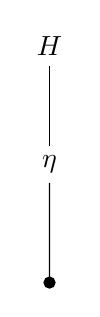
\begin{tikzpicture}
  \node {$H$}
    child {node {$\eta$}
    		child {[fill] circle (2pt)}
    	};
\end{tikzpicture}}
\quad
\begin{tikzpicture}
  \node {$H$} [grow'=up]
    child {node {$\Delta$}
    		child {node {$H$}}
    		child {node {$H$}}
    	};
\end{tikzpicture}
\quad
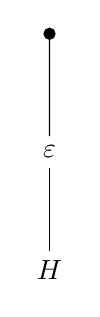
\begin{tikzpicture}[grow'=up]
  \node {$H$}
    child {node {$\varepsilon$}
    		child {[fill] circle (2pt)}
    	};
\end{tikzpicture}
\quad
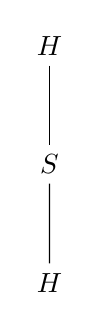
\begin{tikzpicture}
  \node {$H$}
    child {node {$S$}
    		child {node {$H$}}
    	};
\end{tikzpicture}
}

%
%\begin{tikzpicture}
%  \node[fill, circle] {}
%    child {[fill] circle (2pt)}
%    child {[fill] circle (2pt)} {child {[fill] circle (2pt)}}
%    child {[fill] circle (2pt)};
%\end{tikzpicture}

\end{frame}






%============================
% FRAME 2
%============================


\begin{frame}


\frametitle{$Q$-Bialgebras}


\begin{definition}
%{Braided Tensor Product}{•}
Let $A,B$ be algebras with bases $\{ e^v_i \}, \{ e^w_i \}$ respectively. The \Def{braided tensor product} $A \otimes_{Q} B$ with respect to $Q_{ij}$ is defined by
\begin{equation*}
(e^v_i \otimes e^w_j)(e^v_k \otimes e^w_{\ell}) = Q_{jk} (e^v_i e^v_k \otimes e^w_j e^w_\ell).
\end{equation*}
\end{definition}

\begin{definition}
%{•}{•}
If $\otimes_Q$ is a braided tensor product, a \textbf{$Q$-bialgebra} is a bialgebra in the monoidal category of $R$-modules with the $\otimes_Q$ tensor product.
\end{definition}



\end{frame}



\begin{frame}


\frametitle{$Q$-Bialgebras}

\framesubtitle{Example: Spin Statistics}


Let $A$ be a set of elements and $Q_{x y}$ be elements of a ring $k$, for all $x,y \in A$. Then the tensor algebra $T[A]$ has the structure of a $Q$-bialgebra where $\Delta a = a \otimes 1 + 1 \otimes a \in T[A] \otimes_Q T[A]$ for all $a \in A$, and
\begin{equation}
\Delta(xy) = \Delta(x) \Delta(y) = \sum Q_{x_{(2)} y_{(1)}} x_{(1)} y_{(2)} \otimes x_{(2)} y_{(1)}.
\end{equation}

\newthought{Anyons: } In the case that $Q_{xy} = e^{i \phi_{xy}}$, we can interpret the elements $x$ and $y$ as anyons of type $\phi_{xy}$, and the comultiplication satisfies
\begin{equation}
\Delta(xy) = xy \otimes 1 + 1 \otimes xy + x \otimes y + e^{i \phi_{xy}} y \otimes x.
\end{equation}

\end{frame}




%============================
% FRAME 
%============================


\begin{frame}

\frametitle{Wick's Theorem}

\framesubtitle{Standard Product}

\begin{prop}{}{}
%{Wick's Theorem}{wicks-regular-prod}
Let $B$ be a graded $Q$-bialgebra with Laplace pairing $\gen{\cdot, \cdot}$, and let $P \subseteq H$ be the primitive elements. Then
\begin{equation}
\gen{q_1 \ldots q_m,p_1 \ldots p_n} = 
\sum_{j_1, \ldots, j_n} \prod_{\substack{i,a_i,b \\ a_i < j_i \prec a_i \\
j_i \prec b}} Q_{a_i, j_i} (-1)^{\abs{p_i} \abs{q_b}}   \gen{q_{j_i}, p_i}
\end{equation}
if $m = n$, and is zero otherwise. In the above equation $q_i, p_i \in P$, $q_i q_j = Q_{ij} q_j q_i$, and $\prec$ is a partial order defined for every choice of $j_1, \ldots, j_n$, by
\begin{align*}
j_1 \prec \ldots \prec j_n \prec a
\end{align*}
for all $a \notin \{ j_t \}$.
\end{prop}

\end{frame}


\begin{frame}
\frametitle{Precursors}

\framesubtitle{Wick's Theorem}


\textit{On the Hopf algebraic origin of Wick normal-ordering}, Fauser (2001).
\begin{itemize}
\item Proves Wick's theorem in the case of the circle product for $H = \Lambda[V]$.
\end{itemize}

\bigskip

\textit{A quantum field algebra}, Brouder (2002).
\begin{itemize}
\item Proves Wick's theorem for both the ordinary and circle product in the case of $H = S[V]$.

\end{itemize}


\end{frame}



%============================
% FRAME 
%============================
%
%
%\begin{frame}
%
%\frametitle{Wick's Theorem}
%
%\framesubtitle{Standard Product}
%
%
%\begin{align*}
%\gen{q_1 q_2, p_1 p_2} = &(-1)^{\abs{p_1} \abs{q_2}} \gen{q_1, p_1} \gen{q_2, p_2} \\
%&+ Q_{12} (-1)^{\abs{p_1} \abs{q_1}} \gen{q_2, p_1} \gen{q_1, p_2}.
%\end{align*}
%
%
%\begin{align*}
%\langle q_1 q_2 q_3, p_1 &p_2 p_3 \rangle = (-1)^{\abs{p_1} \abs{q_2 q_3} + \abs{p_2} \abs{q_3}} \gen{q_1, p_1} \gen{q_2, p_2} \gen{q_3, p_3} \\ 
%&+ Q_{23} (-1)^{\abs{p_1} \abs{q_2 q_3} + \abs{p_2} \abs{q_2}}  \gen{q_1, p_1} \gen{q_3, p_2} \gen{q_2, p_3} \\
%&+  Q_{12} (-1)^{\abs{p_1} \abs{q_1 q_3} + \abs{p_2} \abs{q_3}} \gen{q_2, p_1} \gen{q_1, p_2}  \gen{q_3, p_3} \\
%&+ Q_{12} Q_{13} (-1)^{\abs{p_1} \abs{q_1 q_3} + \abs{p_2} \abs{q_1}} \gen{q_2, p_1} \gen{q_3, p_2} \gen{q_1, p_3}  \\
%&+ Q_{23} Q_{13} (-1)^{\abs{p_1} \abs{q_1 q_2} + \abs{p_2} \abs{q_2}} \gen{q_3, p_1} \gen{q_1, p_2} \gen{q_2, p_3}  \\
%&+ Q_{12} Q_{13} Q_{23} (-1)^{\abs{p_1} \abs{q_2 q_1} + \abs{p_2} \abs{q_1}} \gen{q_3, p_1} \gen{q_2, p_2} \gen{q_1, p_3} 
%\end{align*}
%
%
%\end{frame}



\begin{frame}

\frametitle{Wick's Theorem}

\framesubtitle{Standard Product}




\begin{align*}
\gen{q_1 q_2, p_1 p_2} = &(-1)^{\abs{p_1} \abs{q_2}} \gen{q_1, p_1} \gen{q_2, p_2} \\
&+ Q_{12} (-1)^{\abs{p_1} \abs{q_1}} \gen{q_2, p_1} \gen{q_1, p_2}.
\end{align*}



\begin{align*}
\langle q_1 q_2 q_3, p_1 p_2 p_3 \rangle = (-1)^{\abs{p_1} \abs{q_2 q_3} + \abs{p_2} \abs{q_3}} \gen{q_1, p_1} \gen{q_2, p_2} \gen{q_3, p_3} + \ldots
\end{align*}




\begin{tabularx}{\textwidth}{llll>{\raggedright\arraybackslash}X}
\toprule
$\gen{-, p_1}$ & $\gen{-, p_2}$ & $\gen{- p_3}$ & Coefficient
\\
\midrule
\colorbox{queer-plum!50}{$1$} & $\text{\colorbox{queer-blue!50}{$2$}}$ & $\text{\colorbox{queer-yellow!50}{$3$}}$ & $(-1)^{\abs{p_1} \abs{\text{\colorbox{queer-blue!50}{$q_2$}} \text{\colorbox{queer-yellow!50}{$q_3$}}} + \abs{p_2} \abs{\text{\colorbox{queer-yellow!50}{$q_3$}}}}$ \\
%
%
\colorbox{queer-plum!50}{$1$} & $\text{\colorbox{queer-yellow!50}{$3$}}$  & $\text{\colorbox{queer-blue!50}{$2$}}$ & $Q_{\text{\colorbox{queer-blue!50}{$2$}} \text{\colorbox{queer-yellow!50}{$3$}}} (-1)^{\abs{p_1} \abs{ \text{\colorbox{queer-yellow!50}{$q_3$}} \text{\colorbox{queer-blue!50}{$q_2$}} } + \abs{p_2} \abs{\text{\colorbox{queer-blue!50}{$q_2$}}}}$ \\
%
%
$\text{\colorbox{queer-blue!50}{$2$}}$ & \colorbox{queer-plum!50}{$1$} & $\text{\colorbox{queer-yellow!50}{$3$}}$  & $Q_{\text{\colorbox{queer-plum!50}{$1$}} \text{\colorbox{queer-blue!50}{$2$}}} (-1)^{\abs{p_1} \abs{\text{\colorbox{queer-plum!50}{$q_1$}} \text{\colorbox{queer-yellow!50}{$q_3$}}} + \abs{p_2} \abs{\text{\colorbox{queer-yellow!50}{$q_3$}}}}$ \\
%
%
$\text{\colorbox{queer-blue!50}{$2$}}$ & $\text{\colorbox{queer-yellow!50}{$3$}}$  & $\text{\colorbox{queer-plum!50}{$1$}}$ & $Q_{\text{\colorbox{queer-plum!50}{$1$}} \text{\colorbox{queer-blue!50}{$2$}} } Q_{\text{\colorbox{queer-plum!50}{$1$}} \text{\colorbox{queer-yellow!50}{$3$}} } (-1)^{\abs{p_1} \abs{ \text{\colorbox{queer-yellow!50}{$q_3$}} \text{\colorbox{queer-plum!50}{$q_1$}} } + \abs{p_2} \abs{\text{\colorbox{queer-plum!50}{$q_1$}}}}$ \\
%
$\text{\colorbox{queer-yellow!50}{$3$}}$  & $\text{\colorbox{queer-plum!50}{$1$}}$ & $\text{\colorbox{queer-blue!50}{$2$}}$ & $Q_{\text{\colorbox{queer-blue!50}{$2$}} \text{\colorbox{queer-yellow!50}{$3$}} } Q_{\text{\colorbox{queer-plum!50}{$1$}} \text{\colorbox{queer-yellow!50}{$3$}} } (-1)^{\abs{p_1} \abs{\text{\colorbox{queer-plum!50}{$q_1$}} \text{\colorbox{queer-blue!50}{$q_2$}}} + \abs{p_2} \abs{\text{\colorbox{queer-blue!50}{$q_2$}}}}$ \\
%
$\text{\colorbox{queer-yellow!50}{$3$}}$  & $\text{\colorbox{queer-blue!50}{$2$}}$ & $\text{\colorbox{queer-plum!50}{$1$}}$ & $Q_{\text{\colorbox{queer-plum!50}{$1$}} \text{\colorbox{queer-blue!50}{$2$}} } Q_{\text{\colorbox{queer-plum!50}{$1$}} \text{\colorbox{queer-yellow!50}{$3$}} } Q_{\text{\colorbox{queer-blue!50}{$2$}} \text{\colorbox{queer-yellow!50}{$3$}} } (-1)^{\abs{p_1} \abs{\text{\colorbox{queer-blue!50}{$q_2$}} \text{\colorbox{queer-plum!50}{$q_1$}}} + \abs{p_2} \abs{\text{\colorbox{queer-plum!50}{$q_1$}}}}$ \\
\end{tabularx}


\end{frame}



%
%
%\begin{frame}
%
%
%
%
%
%\begin{tabularx}{\textwidth}{llll>{\raggedright\arraybackslash}X}
%\toprule
%$\gen{-, p_1}$ & $\gen{-, p_2}$ & $\gen{- p_3}$ & Coefficient
%\\
%\midrule
%$q_1$ & $q_2$ & $q_3$ & $(-1)^{\abs{p_1} \abs{q_2 q_3} + \abs{p_2} \abs{q_3}}$ \\
%$q_1$ & $q_3$ & $q_2$ & $Q_{23} (-1)^{\abs{p_1} \abs{q_2 q_3} + \abs{p_2} \abs{q_2}}$ \\
%$q_2$ & $q_1$ & $q_3$ & $Q_{12} (-1)^{\abs{p_1} \abs{q_1 q_3} + \abs{p_2} \abs{q_3}}$ \\
%$q_2$ & $q_3$ & $q_1$ & $Q_{12} Q_{13} (-1)^{\abs{p_1} \abs{q_1 q_3} + \abs{p_2} \abs{q_1}}$ \\
%$q_3$ & $q_1$ & $q_2$ & $Q_{23} Q_{13} (-1)^{\abs{p_1} \abs{q_1 q_2} + \abs{p_2} \abs{q_2}}$ \\
%$q_3$ & $q_2$ & $q_1$ & $Q_{12} Q_{13} Q_{23} (-1)^{\abs{p_1} \abs{q_2 q_1} + \abs{p_2} \abs{q_1}}$ \\
%\end{tabularx}
%
%
%\end{frame}



%============================
% FRAME 
%============================


\begin{frame}

\frametitle{Circle Product}

%\framesubtitle{Definition}

\begin{definition}{}{}
Let $B$ be a graded bialgebra with Laplace pairing $\gen{\cdot,\cdot}$. The \Def{circle product} on $B$ with respect to $\gen{\cdot,\cdot}$ is
%
\begin{align*}
x \circ y &=  \sum (-1)^{\abs{x_{(2)}} \abs{y_{(1)}}} \gen{x_{(1)}, y_{(1)}} x_{(2)} y_{(2)}. 
\end{align*}

\end{definition}


\end{frame}




%============================
% FRAME 
%============================


\begin{frame}

\frametitle{Wick's Theorem}

\framesubtitle{Circle Product}

\begin{prop}{Wick's Theorem for the Circle Product}{wicks-circle-prod}
Let $B$ be a bialgebra with Laplace pairing $\gen{\cdot, \cdot}$, and let $P \subseteq H$ be the primitive elements. Then
\begin{equation}
\gen{\bar{q}^\circ, \bar{p}^\circ} = \sum_{k, \ell} \prod_{\substack{x_i < x_j \prec x_{j+t} \\ x_a < x_b \prec x_a}} (-1)^{\abs{x_a} \abs{x_b}} \gen{x_i,x_j} \prod_{x_{j_k}, x_{j_\ell} \prec c < x_r \prec c < p_1} Q_{c,r}
\end{equation}
if $\abs{\bar{q}^\circ} + \abs{\bar{p}^\circ}$ is even, and is zero otherwise.
\end{prop}

where 
\begin{align*}
q_1 < \ldots < q_m &< p_1 < \ldots < p_n \\
q_{i_1} \prec q_{i_2}  \prec \ldots \prec q_{j_1} &\prec  q_{j_2} \prec \ldots \prec x \\
p_{k_1} \prec p_{k_2} \prec \ldots \prec p_{\ell_1} &\prec p_{\ell_2} \prec \ldots \prec x \\
q_{i_1} \prec \ldots q_{j_1} \prec \ldots \prec p_{k_1} \prec \ldots \prec p_{\ell_1} &\prec \ldots \prec q_{r_1} \prec p_{r_1} \prec \ldots \prec q_{r_k} \prec p_{r_k}.
\end{align*}

\end{frame}


%============================
% FRAME 
%============================


\begin{frame}

\frametitle{Wick's Theorem}

\framesubtitle{Circle Product}

%\begin{align*}
%\gen{q_1, p_1 \circ p_2 \circ p_3} &= \gen{q_1, p_1} \gen{p_2, p_3} + (-1)^{\abs{p_2} \abs{p_1}} \gen{q_1, p_2} \gen{p_1, p_3} \\
%&+ (-1)^{\abs{p_3} \abs{p_1 p_2}} \gen{q_1, p_3} \gen{p_1, p_2}.
%\end{align*}
%
%
%\begin{tabularx}{\textwidth}{lll>{\raggedright\arraybackslash}X}
%\toprule
%$\gen{-, -}$ & $\gen{-, -}$ & Coefficient
%\\
%\midrule
%\colorbox{queer-plum!50}{$q_1$} \colorbox{queer-blue!50}{$p_1$} & \colorbox{queer-yellow!50}{$p_2$} \colorbox{queer-lavender!50}{$p_3$} & 1 \\
%%
%%
%\colorbox{queer-plum!50}{$q_1$} \colorbox{queer-yellow!50}{$p_2$} & \colorbox{queer-blue!50}{$p_1$} \colorbox{queer-lavender!50}{$p_3$} & $(-1)^{\abs{\text{\colorbox{queer-yellow!50}{$p_2$}}} \abs{ \text{\colorbox{queer-blue!50}{$p_1$}}} }$ \\
%%
%%
%\colorbox{queer-plum!50}{$q_1$} \colorbox{queer-lavender!50}{$p_3$} & \colorbox{queer-yellow!50}{$p_2$} \colorbox{queer-blue!50}{$p_1$} & $(-1)^{\abs{\text{\colorbox{queer-lavender!50}{$p_3$}}} \abs{ \text{\colorbox{queer-blue!50}{$p_1$} \text{\colorbox{queer-yellow!50}{$p_2$}  }}} }$ \\
%%
%%
%
%\end{tabularx}


\begin{align*}
\gen{q_1 \circ q_2 \circ q_3, p_1} &= \gen{q_1, q_2} \gen{q_3, p_1} + Q_{23} (-1)^{\abs{q_3} \abs{q_2}} \gen{q_1, q_3} \gen{q_2, p_1} \\
&+ (-1)^{\abs{p_1} \abs{q_2 q_3} } \gen{q_1, p_1} \gen{q_2, q_3}.
\end{align*}

\bigskip

\bigskip

\begin{tabularx}{\textwidth}{lll>{\raggedright\arraybackslash}X}
\toprule
$\gen{-, -}$ & $\gen{-, -}$ & Coefficient
\\
\midrule
\colorbox{queer-plum!50}{$q_1$} \colorbox{queer-blue!50}{$q_2$} & \colorbox{queer-yellow!50}{$q_3$} \colorbox{queer-lavender!50}{$p_1$} & 1 \\
%
%
\colorbox{queer-plum!50}{$q_1$} \colorbox{queer-yellow!50}{$q_3$} & \colorbox{queer-blue!50}{$q_2$} \colorbox{queer-lavender!50}{$p_1$} & $(-1)^{\abs{\text{\colorbox{queer-yellow!50}{$q_3$}}} \abs{ \text{\colorbox{queer-blue!50}{$q_2$}}} } Q_{\text{\colorbox{queer-blue!50}{$q_2$}} \text{\colorbox{queer-yellow!50}{$q_3$}} } $ \\
%
%
\medskip
\colorbox{queer-plum!50}{$q_1$} \colorbox{queer-lavender!50}{$p_1$} & \colorbox{queer-yellow!50}{$q_3$} \colorbox{queer-blue!50}{$q_2$} & $(-1)^{\abs{\text{\colorbox{queer-lavender!50}{$p_1$}}} \abs{ \text{\colorbox{queer-blue!50}{$q_2$} \text{\colorbox{queer-yellow!50}{$q_3$}  }}} }  $ \\
%
%
\end{tabularx}




\end{frame}



%============================
% FRAME 
%============================


\begin{frame}

\frametitle{Wick's Theorem}



\begin{align*}
\gen{\text{\colorbox{queer-plum!50}{$q_1$}} \text{\colorbox{queer-blue!50}{$q_2$}}, \text{\colorbox{queer-yellow!50}{$p_1$}} \text{\colorbox{queer-lavender!50}{$p_2$}}} = &(-1)^{\abs{\text{\colorbox{queer-yellow!50}{$p_1$}}} \abs{\text{\colorbox{queer-blue!50}{$q_2$}}}} \gen{\text{\colorbox{queer-plum!50}{$q_1$}}, \text{\colorbox{queer-yellow!50}{$p_1$}}} \gen{\text{\colorbox{queer-blue!50}{$q_2$}}, \text{\colorbox{queer-lavender!50}{$p_2$}}} \\
&+ Q_{\text{\colorbox{queer-plum!50}{$1$} \colorbox{queer-blue!50}{$2$}}} (-1)^{\abs{\text{\colorbox{queer-yellow!50}{$p_1$}}} \abs{\text{\colorbox{queer-plum!50}{$q_1$}}}} \gen{\text{\colorbox{queer-blue!50}{$q_2$}}, \text{\colorbox{queer-yellow!50}{$p_1$}}} \gen{\text{\colorbox{queer-plum!50}{$q_1$}}, \text{\colorbox{queer-lavender!50}{$p_2$}}}.
\end{align*}



\begin{align*}
\gen{\text{\colorbox{queer-plum!50}{$q_1$}} \circ \text{\colorbox{queer-blue!50}{$q_2$}}, \text{\colorbox{queer-yellow!50}{$p_1$}} \circ \text{\colorbox{queer-lavender!50}{$p_2$}}} &= (-1)^{\abs{\text{\colorbox{queer-yellow!50}{$p_1$}}} \abs{\text{\colorbox{queer-blue!50}{$q_2$}}}} \gen{\text{\colorbox{queer-plum!50}{$q_1$}}, \text{\colorbox{queer-yellow!50}{$p_1$}}} \gen{\text{\colorbox{queer-blue!50}{$q_2$}}, \text{\colorbox{queer-lavender!50}{$p_2$}}} \\
&+ \gen{\text{\colorbox{queer-plum!50}{$q_1$}}, \text{\colorbox{queer-blue!50}{$q_2$}}} \gen{\text{\colorbox{queer-yellow!50}{$p_1$}}, \text{\colorbox{queer-lavender!50}{$p_2$}}} \\
&+ (-1)^{\abs{\text{\colorbox{queer-lavender!50}{$p_2$}}} \abs{\text{\colorbox{queer-blue!50}{$q_2$}} \text{\colorbox{queer-yellow!50}{$p_1$}}}} \gen{\text{\colorbox{queer-plum!50}{$q_1$}}, \text{\colorbox{queer-lavender!50}{$p_2$}}} \gen{\text{\colorbox{queer-blue!50}{$q_2$}}, \text{\colorbox{queer-yellow!50}{$p_1$}}}.
\end{align*}


\end{frame}





%============================
% FRAME
%============================


\begin{frame}

\frametitle{Hopf-Frobenius Modules}

\framesubtitle{Definition}

%{Hopf-Frobenius Module}{hopf-frob}
A \Def{left Hopf-Frobenius module} is a pair $(H,F)$ where $H$ is a Hopf algebra, and $F$ is a Frobenius algebra such that

\medskip
\begin{itemize}
\item \fbox{Module: } $F$ has the structure of a left $H$-module.

\medskip

\item \fbox{Weak Cartan: }   $\sum (-1)^{\abs{x} \abs{g_{(2)}}} \gen{g_{(1)} x, g_{(2)} y} = \varepsilon_H(g) \gen{x,y}$.

\medskip 

\item \fbox{Antipode Condition: }  $\gen{g x, y} = (-1)^{\abs{g} \abs{x}} \gen{x, S(g) y}. $
\end{itemize}

\medskip
for all $g \in H$, $x,y \in F$.



\end{frame}




%============================
% FRAME
%============================


\begin{frame}

\frametitle{Hopf-Frobenius Modules}

\framesubtitle{Examples}


\begin{tabularx}{\textwidth}{ll|ll>{\raggedright\arraybackslash}X}
\toprule
Frobenius & & Hopf
\\
\midrule
& & \\
Vector space & $V$ & Lie algebra & $U[\mathfrak{g}]$ \\
Vector space & $V$ & Lie group & $k G$ \\
Functions (Haar) & $L(G)$ & Compact group & $\mathbb{R} G$
\\
Functions & $C^{\infty}_c(\mathbb{R}^n)$ & Derivatives & $U \left[ \operatorname{Der}(C^{\infty}_c(\mathbb{R}^n)) \right]$ \\
&& \\
\bottomrule
\end{tabularx}




\end{frame}




%============================
% FRAME
%============================


\begin{frame}

\frametitle{Lie Algebra of a Hopf Algebra}

\framesubtitle{Definition}

%\begin{definition}
%{Lie Algebra of a Hopf Algebra}{•}
Let $H$ be a Hopf algebra. The \Def{Lie algebra associated to $H$} is the vector space
\begin{equation}
\mathfrak{L}_H \equiv \left\lbrace \sum_i \alpha_i (x - S(x)) \mid x \in H, S^2(x) = x, \alpha_i \in k \right\rbrace,
\end{equation}
with the commutator bracket.

%\end{definition}

\end{frame}



\begin{frame}
\frametitle{Precursors}

\framesubtitle{Lie Algebra of a Hopf Algebra}



\textit{On a certain Lie algebra defined by a finite group}, Cohen and Taylor (2007).

\begin{itemize}
\item They study the Lie algebra in the case $H = kG$, for a \textit{finite group} $G$, referring to it as the \Def{Plesken Lie algebra}, named for the mathematician who brought it to their attention.
\end{itemize}

\bigskip

\textit{Group algebras of finite groups as lie algebras}, Marin (2010).

\begin{itemize}
\item Considers $g - \chi(g) g^{-1}$ for a multiplicative character $\chi$.
\end{itemize}


\end{frame}





%============================
% FRAME
%============================


\begin{frame}

\frametitle{Hopf-Frobenius Modules}

\framesubtitle{Lie Algebra of Hopf Algebra}


%in the case that we start with a universal enveloping algebra, we recover the lie algebra


\begin{prop}{}{lie-alg-matches}
Let $G$ be a Lie group over a field $k$ that satisfies the following property: 

\begin{itemize}
\item There exists a collection of non-degenerate bilinear forms $\{ \gen{\cdot \cdot}_\alpha \}$ on a vector space $V$ such that 
\begin{align*}
G = \{ g \in \operatorname{End}(V) \mid \gen{g x, gy}_\alpha = \gen{x,y}_\alpha, \text{ for all } \gen{\cdot, \cdot}_\alpha \}
\end{align*}
and the Lie algebra of $G$ is
\begin{align*}
\mathfrak{g} = \{ A \in \operatorname{End}(V) \mid \gen{Ax, y}_{\alpha} = - \gen{x, Ay}_{\alpha}, \text{ for all } \gen{\cdot, \cdot}_\alpha \}.
\end{align*}
\end{itemize}

Then $\mathfrak{L}_G \cong \mathfrak{g}$.
%
%non-degenerate bilinear form
%
%Let $G$ be one of the following Lie groups: $O(n), U(n), GL(n), SL(n), Sp(n), O(p,q)$. Then $\mathfrak{L}_G$ matches the corresponding classical Lie algebra.
\end{prop}


\newthought{Examples: } $U(n), O(n), Sp(n), O(m,n)$.


\end{frame}



%============================
% FRAME
%============================


\begin{frame}

\frametitle{Lie Group of a Hopf-Frobenius Module}

\framesubtitle{Definition}


%\begin{definition}{Lie Group of a Hopf-Frobenius Module}{}
Let $(H,F)$ be a Hopf-Frobenius module, $\{ \gen{-,-}_\alpha \}$ be a collection of Frobenius forms on $F$, and $U$ be the subalgebra generated by the primitive elements of $H$. The set
\begin{align*}
\cat{G}^H_F \equiv \{ g \in U/\operatorname{ann} F \mid &\gen{g x, gy}_\alpha = \gen{S(g) x, S(g) y}_\alpha = \gen{x,y}_\alpha \\
 &\text{ and } \gen{S(g) x, y}_\alpha = \gen{x, g y}_\alpha, \; \text{for all } \alpha \}
\end{align*}
forms a group, called the \Def{Lie group of $(H,F)$}.
%\end{definition}


\end{frame}




%============================
% FRAME
%============================


\begin{frame}

\frametitle{Lie Correspondence}


\begin{prop}{}{}
Let $G$ be one of the following Lie groups with its standard representation $\rho$ on the relevant vector space $F$ with bilinear forms $\{ \gen{\cdot, \cdot}_\alpha \}$:
\begin{align*}
\{ O(n), SO(n), U(n) \mid n > 2 \} \cup \{ Sp(n) \} \cup \{ F_4 \}.
\end{align*}
Let $\mathfrak{g}$ be the corresponding Lie algebra. Then
\begin{align*}
\cat{G}_F^{U[\mathfrak{g}]} \cong G
\end{align*}
as topological groups.
\end{prop}


\end{frame}

%
%%============================
%% FRAME
%%============================
%
%
%\begin{frame}
%
%\frametitle{Lie Correspondence}
%
%\framesubtitle{Exceptional Lie Group}
%
%
%
%\begin{example}{Lie Group: $F_4$}
%%{lie-group-f4}
%
%The exceptional Lie group $F_4$ is the isometry group of the octonions. We can view the octonions as a non-associative Frobenius algebra over the real numbers. The above construction will yield
%\begin{equation}
%\cat{G}_{\mathbb{O}}^{U[\mathfrak{g}]} \cong F_4.
%\end{equation}
%
%
%%This is the isometry group of the octonions (well it's really for the projective octonions, so it's like $so(n)$)
%
%
%
%\end{example}
%
%
%\end{frame}
%


%============================
% FRAME
%============================


\begin{frame}

\frametitle{Creation/Annihilation Operators}

Given a coalgebra $C$ with basis $\{ x_i \}$, Joni and Rota defined creation/annihilation operators with respect to the basis by
\begin{align*}
a^{\dagger}_j x_k &= \sum_i (i \mid j,k) x_i \\
a_j x_k &= \sum_i (k \mid j,i) x_i.
\end{align*}
where $(i \mid j,k)$ is the coefficient of $x_j \otimes x_k$ in $\Delta x_i$.

\newthought{Fock space: } Let $S[A]$ be the symmetric algebra over the algebra $A$, with the comultiplication
\begin{align*}
\Delta f^n = \sum_k \sqrt{\dfrac{n!}{(n-k)!}} f^{k} \otimes f^{n-k}.
\end{align*}



\end{frame}



\begin{frame}


\frametitle{Creation/Annihilation Operators}

Taking the creation/annihilation operators on $S[A]$, we obtain the ordinary behaviour of the creation/annihilation operators in quantum field theory:
\begin{equation}
\begin{split}
a_f^{\dagger} f^n &= \sqrt{n+1} f^{n+1}. \\
a_f f^n &= \sqrt{n} f^{n-1}.
\end{split}
\end{equation}
%This is precisely the behaviour of the ordinary creation/annihilation operators from quantum theory.



\end{frame}


%============================
% FRAME
%============================


\begin{frame}

\frametitle{Hopf Quantization}

\framesubtitle{Deformation Quantization}

\newthought{Poisson algebra: } Let $M$ be a symplectic manifold and let $\mathfrak{p} = C^\infty(M)$ be the Poisson algebra of functions over the manifold. 

\newthought{Quantization: } Take $H_c = T[\mathfrak{p}]$ with the following coproduct and Laplace pairing
\begin{align*}
\Delta_x \phi &= 1 \otimes \phi + \phi \otimes 1 - \phi(x) 1 \otimes 1
\end{align*}
for some fixed $x \in M$. Given an arbitrary Laplace pairing $\gen{-,-}$, the commutator with respect to the circle product can be identified with the \Def{Moyal bracket}:
%
\begin{equation}
[\phi, \psi]_x^{\gen{\cdot, \cdot}} = [\phi, \psi] + (\gen{\phi, \psi} - \gen{\psi, \phi}) 1.
\end{equation}

\end{frame}



%============================
% FRAME
%============================



\begin{frame}


\frametitle{Hopf Quantization}

\framesubtitle{Bosonic Fock Space Quantization}



\newthought{Fock space: } Let $A$ be an algebra and take the symmetric algebra $S[A]$.

\newthought{Operators: } Let $H$ be the tensor algebra creation and annihilation operators $\{ a_f, a_f^\dagger \}$.

\newthought{Quantization: } Taking the following Laplace pairing makes the circle product into the \textbf{normal ordering} on creation/annihilation operators:
%
\begin{align*}
\gen{a_f, a_g^\dagger} &= \delta_{f,g} \\
\gen{a_f^{\dagger}, a_g} &= 0.
\end{align*}



\end{frame}




%============================
% FRAME
%============================



\begin{frame}


\frametitle{Hopf-Frobenius Quantum Field Theory}

\framesubtitle{Definition}


%\begin{definition}
%{Hopf-Frobenius Quantum Field Theory}{hopf-frob-qft}
A \Def{Hopf-Frobenius quantum field theory} is a collection of three Hopf-Frobenius modules, $(H_f, F_f)$, $(H_{ST}, F_{ST})$, and $(H_I, F_I)$ which are meant to model the local functions, spacetime, and internal structure of the theory, respectively.
%\end{definition}


\newthought{Fields: } A classical field in an HFQFT is an element of the tensor product of Frobenius algebras
\begin{align*}
\sum_i f_{ij}(x) \otimes e_i \otimes \theta_j \in F_f \otimes F_{ST} \otimes F_I.
\end{align*}


\end{frame}





%============================
% FRAME
%============================


\begin{frame}


\frametitle{Connections}


%\begin{definition}
%{Connection on a Frobenius Algebra}{}
Let $F_f$ be a fixed Frobenius algebra of functions. Given a Frobenius algebra $F_2$, a \Def{$F_f$-connection on $F_2$} is a pair $(\nabla, F_1)$, where $F_1$ is another Frobenius algebra and $\nabla$ is a linear morphism 
\begin{equation}
\nabla: F_2 \to F_f \otimes F_1 \otimes F_2.
\end{equation}
%When $F_f$ and $F_2$ are clear, we will simply refer to $\nabla$ as the connection.

%\end{definition}



\end{frame}


%============================
% FRAME
%============================


\begin{frame}


\frametitle{Covariant Derivative}

%\begin{definition}
%{Covariant Derivative}{•}
Let $\nabla: F_2 \to F_f \otimes F_1 \otimes F_2$ be a connection, and $d: F_f \to F_f \otimes F_1$ a linear map. The \Def{covariant derivative with respect to $\nabla$} is the map
\begin{align*}
D_\nabla: F_f \otimes F_2 \to F_f \otimes F_1 \otimes F_2
\end{align*}
given by
\begin{align*}
D_\nabla(\sum_i f_i(x) \otimes \theta_i) &= \sum_i d f_i(x) \otimes \theta_i \\
&+ \sum_i f_i(x) (\nabla \theta_i)_{(1)} \otimes (\nabla \theta_i)_{(2)} \otimes (\nabla \theta_i)_{(3)}.
\end{align*}
%\end{definition}


\end{frame}



%============================
% FRAME
%============================


\begin{frame}


\frametitle{Connections}

\framesubtitle{Example: Spacetime}

A \Def{connection on spacetime} will be a connection of the form
\begin{align*}
\nabla: F_{ST} \to F_f \otimes F_{ST} \otimes F_{ST}.
\end{align*}

Say that our spacetime Frobenius algebra is $\mathbb{R}^4$ with a chosen basis $\{ e_0, \ldots, e_3 \}$, where $e_0$ corresponds to the time direction. Expanding the connection in the basis, we have
\begin{equation}
\nabla e_j = \sum_{ik} \Gamma_{ij}^k(x) \otimes e_i \otimes e_k.
\end{equation}
The functions $\Gamma_{ij}^k(x)$ are called the \Def{Christoffel symbols}.


\newthought{Covariant derivative: } Our covariant derivative will take the form
\begin{align*}
D_\nabla f &= df + \sum_i f_i \otimes \nabla e_i \\
&= \sum_{ij} \partial_j f_i \otimes e_j \otimes e_i + \sum_{ijk} f_i(x) \Gamma_{ji}^k (x) \otimes e_j \otimes e_k.
\end{align*}

\end{frame}



%============================
% FRAME
%============================


\begin{frame}


\frametitle{Connections}

\framesubtitle{Example: Gauge Field}

A \Def{gauge connection} is a connection of the form
\begin{align*}
\nabla: F_{I} \to F_f \otimes F_{ST} \otimes F_{I}.
\end{align*}


\newthought{Gauge Potential: } If we expand out in a basis, we can write
\begin{equation}
\nabla e_j = \sum_{ik} A_{ij}^k(x) \otimes e_i \otimes \theta_k.
\end{equation}
The terms $A_{ij}^k(x)$ are referred to in physics as the \textbf{gauge field} of the gauge connection

%\footnote{Strictly speaking, the gauge field is normally taken to be $i g A_{ab}^c(x)$, where $g$ is called the \textit{coupling parameter}.}.


\end{frame}


%============================
% FRAME
%============================


\begin{frame}


\frametitle{Gauge Theory: $U(1)$}


\newthought{Internal symmetry: } $F_I$ is one-dimensional. Say that $F_I$ is spanned by the vector $\theta$. Then $U(1)$ acts on the fields as
\begin{equation}
f \otimes e_i \otimes \theta \to f \otimes e_i \otimes e^{i \phi} \theta.
\end{equation}
%Using the isomorphism $F_f \otimes F_{ST} \otimes F_I \cong F_f \otimes F_{ST}$, we can think of the action of $U(1)$ as scalar multiplication on $F_f \otimes F_{ST}$ by a complex phase.

%\newthought{Physics notation: } In physics notation, the dimensions of $F_{ST}$ are normally encoded in a subscript or superscript, so we would write the action of $U(1)$ as
%\begin{align*}
%\phi_\mu \to e^{i \theta} \phi_\mu.
%\end{align*}
%In the case that $\phi$ is a scalar field, the index is suppressed, so $\phi \to e^{i \theta} \phi$.

\newthought{Connection: } Our gauge connection will be a map 
\begin{align*}
\nabla: F_I \to F_f \otimes F_{ST} \otimes F_I.
\end{align*}
Applying our isomorphism $F_{I} \cong k$, where $k$ is the underlying field, we have that our connection can be thought of as a map
\begin{equation}
\nabla: k \to F_f \otimes F_{ST}.
\end{equation}
This is the same data as an element of $F_f \otimes F_{ST}$, which we think of as a vector field. This element is called the \Def{electromagnetic four-potential}.


\end{frame}



\begin{frame}


\frametitle{Gauge Theory: $U(1)$}


\newthought{Physics notation: } The electromagnetic four-potential is normally denoted $A_\mu$. In components, we have
\begin{align*}
\nabla \theta = \sum_\mu A_\mu(x) \otimes e_\mu \otimes \theta.
\end{align*}

\newthought{Covariant derivative: } The covariant derivative corresponding to $A_\mu$ will be
\begin{align*}
D_\nabla \phi &= \sum_{j} \partial_j \phi \otimes e_j \otimes \theta + \sum_{i} \phi A_i(x) \otimes e_i \otimes \theta.
\end{align*}
Using the isomorphism $F_I \cong k$, we can view the covariant derivative as
\begin{align*}
D_\nabla \phi = \sum_{i} \partial_i \phi \otimes e_i + \phi(x) A_i(x) \otimes e_i.
\end{align*}
\end{frame}

%============================
% FRAME
%============================


\begin{frame}


\frametitle{Gauge Theory: $SU(3)$}


\newthought{Connection: } $F_I \cong \mathbb{C}^3$. The \Def{gluon field} $G_{ij}^k(x)$ comes from the connection:
\begin{equation}
\nabla \theta_i = \sum G_{ij}^k(x) \otimes e_j \otimes \theta_k.
\end{equation}

\newthought{Covariant derivative: } 
\begin{align*}
D_\nabla \varphi 
&= \sum_{ij} \partial_j \varphi_i \otimes e_j \otimes \theta_i + \sum_{ijk} \varphi_i(x)  G_{ij}^k(x) \otimes e_j \otimes \theta_k.
\end{align*}
Or, expressed in a form more familiar to physicists, we have, in each dimension $e_\mu$,
\begin{align*}
D_\mu \varphi
&= \sum_{i} \partial_\mu \varphi_i \otimes \theta_i + \sum_{ik} \varphi_i(x)  G_{i\mu}^k(x) \otimes \theta_k \\
&= \partial_\mu \varphi + G_\mu^k \cdot \varphi
\end{align*}
where, in the last line we are implicitly considering $\varphi$ to be a three-dimensional vector.


\end{frame}


%============================
% FRAME
%============================




\begin{frame}
\frametitle{Hopf-Frobenius Wightman Axioms}\footnotetext{The Wightman axioms were introduced in \textit{PCT, spin and statistics, and all that} (2000).}
%\framesubtitle{Relativistic Quantum Mechanics}




A (weak) Hopf-Frobenius-Wightman QFT is a collection of Hopf algebras ($B(F_{\text{state}}), k SL(2)$)  and Frobenius algebras ($F_{\text{state}}, \cat{S}, \mathbb{R}^{1,3}$)  such that

\bigskip

\begin{enumerate}


\item \fbox{States and Evolution: } $(k SL(2),F_{\text{state}})$ forms a Hopf-Frobenius module.

\item \fbox{Vacuum: } There is a unit $1 \in F_{\text{state}}$, which is the unique element preserved by $k SL(2)$.

\item \fbox{Fields: } Quantum fields are linear maps $\cat{S} \to B(F_{\text{state}})$ and form a Frobenius algebra $F_{\text{field}}$.

\item \fbox{Field Transformations: } $(k SL(2),F_{\text{field}})$ forms a Hopf-Frobenius module.





\end{enumerate}


\end{frame}

%
%
%
%\begin{frame}
%\frametitle{Hopf-Frobenius Wightman Axioms}
%\framesubtitle{Other Conditions}
%
%\begin{enumerate}
%
%\item \fbox{Dense Subset: } We can view $F_{\text{state}}$ as all of $D$.
%
%
%\item \fbox{Cyclic Vacuum: } The image of polynomials in $\phi_i(f)$ on $\ket{0}$ is dense in $X$.
%
%
%\item \fbox{Spectral Condition: } We can write $U(1,a) = \exp(i P^{\mu} a_\mu)$ and the eigenvalues of $P$ satisfy $p_0^2 - \sum_{i=1}^3 p_i^2 > 0$ and $p^0 > 0$.
%
%
%\item \fbox{Causality: }  If $f,g \in \cat{S}$ have spacelike supports ($f(x) g(y) = 0$ for all $x,y$ with $d(x,y) \geq 0$) then $[\phi_i (f), \phi_j (g)]_{\pm}(v) = 0$ for all $v \in D$.
%
%
%\end{enumerate}
%\end{frame}
%




%============================
% FRAME
%============================


\begin{frame}

\frametitle{Operad of Operad Algebras}

\begin{prop}{The Operad of Operad Algebras}{operad-of-operad-alg-gen}
Let $\cat{V}$ be a symmetric monoidal category with all small coproducts and let $\cat{O}$ be a coloured operad in $\cat{V}$. For any small category, $\cat{C}$, there exists an operad $\cat{O}^{\cat{C}}$ in $\cat{V}$ whose algebras are the functors 
\begin{equation*}
F: \cat{C} \to \cat{O} \text{-Alg}.
\end{equation*}
\end{prop}

\begin{prop}{Properad of Properad Algebras}{prop-of-prop-algs}
Let $\cat{P}$ be a coloured properad in a closed monoidal category with all small coproducts $\cat{V}$. For any small category $\cat{C}$, there exists a properad $\cat{P}^{\cat{C}}$ whose algebras are the functors
\begin{equation*}
F: \cat{C} \to \cat{P}\text{-Alg}.
\end{equation*}
\end{prop}


\end{frame}


\begin{frame}
\frametitle{Precursors}

\framesubtitle{Operad of Operad Algebras}


\textit{Colored Operads}, Yau (2017).

\begin{itemize}
\item The construction of $\cat{O}^{\cat{C}}$ is left as an exercise.
\end{itemize}


\bigskip



\textit{Operads for algebraic quantum field theory}, Benini, Schenkel, Woike (2021).

\begin{itemize}
\item $\cat{O}^{\cat{C}}$ is constructed in the case that $\cat{O}$ is the associative operad.

\end{itemize}





\end{frame}






%============================
% FRAME
%============================




\begin{frame}

\frametitle{Orthogonal Category}

Let $\cat{C}$ be a small category. An \Def{orthogonality relation} $\perp$ on $\cat{C}$ is a relation on pairs of morphisms in $\cat{C}$ such that if $f \perp g$
then $f$ and $g$ have the same codomain, and required to satisfy
\begin{itemize}
\item If $f \perp g$ then $g \perp f$.

\item If $g \perp h$ then $fg \perp fh$ for all composable $f$.

\item If $g_1 \perp g_2$ then $g_1 h \perp g_2 k$ for all composable $h,k$.
\end{itemize}

\medskip

An \Def{orthogonal category} is a small category $\cat{C}$ with an orthogonality relation $\perp$.


\end{frame}


\begin{frame}

\frametitle{Properad of Laplace Hopf AQFTs}\footnotetext{AQFTs were introduced in \textit{An algebraic approach to quantum field theory} Haag and Kastler (1964).}


Let $(\cat{C}, \perp)$ be an orthogonal category. A \Def{Laplace Hopf algebraic quantum field theory} is a functor
\begin{align*}
F: \cat{C} \to \cat{LB}(\cat{V})
\end{align*}
where $\cat{LB}(\cat{V})$ is the category of Laplace bialgebras on a symmetric monoidal category $\cat{V}$, such that the following \textbf{causality diagram} commutes:

\medskip

\begin{center}
\begin{tikzcd}[ampersand replacement=\&]
F(A) \otimes F(B) \arrow[r, "F(f) \otimes F(g)"] \arrow[d, swap, "F(f) \otimes F(g)"] \& F(C) \otimes F(C) \arrow[r, "\tau"] \& F(C) \otimes F(C) \arrow[d, "\mu"] \\
F(C) \otimes F(C) \arrow[rr, swap, "\mu"]  \& \& F(C)
\end{tikzcd}
\end{center}

\medskip 

whenever $f \perp g$.

\end{frame}




\end{document}